% Compile with: pdflatex report.tex
\documentclass[10pt,a4paper]{article}

\usepackage[a4paper,margin=1in]{geometry}
\usepackage[T1]{fontenc}
\usepackage[utf8]{inputenc}
\usepackage{lmodern}
\usepackage{microtype}
\usepackage{amsmath}
\usepackage{amssymb}
\usepackage{array}
\usepackage{booktabs}
\usepackage{enumitem}
\usepackage{graphicx}
\usepackage{hyperref}
\usepackage{caption}
\usepackage{subcaption}
\usepackage{tikz}
\usepackage{pgfplots}
\usepackage{titlesec}
\usepackage{xcolor}
\usepackage{fancyhdr}
\usepackage{lastpage}
\usepackage{float}

\usetikzlibrary{arrows.meta,positioning,calc,fit,backgrounds,shapes.geometric}
\pgfplotsset{compat=1.18}

\definecolor{brandblue}{HTML}{1D4ED8}
\definecolor{brandgreen}{HTML}{047857}
\definecolor{brandorange}{HTML}{C2410C}
\definecolor{brandpurple}{HTML}{6D28D9}
\definecolor{softblue}{HTML}{EFF6FF}
\definecolor{softgreen}{HTML}{ECFDF5}
\definecolor{softorange}{HTML}{FFF7ED}
\definecolor{softpurple}{HTML}{F5F3FF}
\definecolor{linegray}{HTML}{475569}

\hypersetup{
  colorlinks=true,
  linkcolor=brandblue,
  urlcolor=brandblue,
  citecolor=brandblue,
  pdftitle={GATEWay - Comprehensive Technical Report},
  pdfauthor={Technical Team},
}

\titleformat{\section}{\Large\bfseries\color{brandblue}}{\thesection.}{0.5em}{}
\titleformat{\subsection}{\large\bfseries\color{brandgreen}}{\thesubsection}{0.4em}{}
\titleformat{\subsubsection}{\normalsize\bfseries\color{brandpurple}}{\thesubsubsection}{0.3em}{}

\setlength{\parindent}{0pt}
\setlength{\parskip}{6pt}
\setlist[itemize]{leftmargin=*, itemsep=3pt, topsep=3pt}
\setlist[enumerate]{leftmargin=*, itemsep=3pt, topsep=3pt}

\newcommand{\tech}[1]{\texttt{\color{brandblue}#1}}
\newcommand{\project}{GATEWay}
\newcommand{\formula}[1]{\textbf{\textit{#1}}}

% Header and Footer
\pagestyle{fancy}
\fancyhf{}
\rhead{GATEWay - Technical Report}
\lhead{\thepage/\pageref{LastPage}}
\cfoot{Prepared: April 2026}

\tikzset{
  flow/.style={
    rectangle,
    rounded corners=4pt,
    draw=brandblue!70,
    fill=softblue,
    thick,
    align=center,
    minimum height=0.82cm,
    minimum width=2.2cm,
    font=\footnotesize
  },
  store/.style={
    rectangle,
    rounded corners=4pt,
    draw=brandgreen!70!black,
    fill=softgreen,
    thick,
    align=center,
    minimum height=0.82cm,
    minimum width=2.2cm,
    font=\footnotesize
  },
  decision/.style={
    diamond,
    draw=brandorange!80!black,
    fill=softorange,
    thick,
    align=center,
    aspect=1.9,
    inner sep=1.5pt,
    font=\footnotesize
  },
  insight/.style={
    rectangle,
    rounded corners=4pt,
    draw=brandpurple!80,
    fill=softpurple,
    thick,
    align=center,
    minimum height=0.82cm,
    minimum width=2.2cm,
    font=\footnotesize
  },
  line/.style={-{Latex[length=2mm]}, thick, draw=linegray},
  group/.style={draw=linegray!60, dashed, rounded corners=6pt, inner sep=5pt}
}

\title{

\Huge\textbf{\project}\\
\Large An Intelligent GATE DA Preparation Platform\\
\normalsize With Advanced Recommendation Engines, Analytics, and Predictive Scoring
}
\author{Khethavath Sunil Naik \\ 12341170}
\date{\today}

\begin{document}
\maketitle

\begin{abstract}
\project{} is a sophisticated, classroom-aware educational intelligence platform designed specifically for GATE (Graduate Aptitude Test in Engineering) Data Analytics (DA) preparation. The system provides dual-mode experiences: a comprehensive student workspace for structured practice, adaptive testing, personalized coaching, and performance tracking, coupled with an advanced teacher command center for classroom orchestration, assignment management, learner monitoring, and intervention planning. 

The platform's core innovation lies in its unified architecture that seamlessly integrates multiple specialized recommendation engines, a telemetry-driven analytics layer powered by Supabase, graph-based adaptive sequencing, intelligent rule-based coaching, comprehensive performance analytics, and a novel predictive scoring model. This report provides a detailed technical exposition of the complete system architecture, mathematical formulas underlying key recommendations, all data models, recommendation engine implementations, teacher analytics pipelines, and the comprehensive GATE score prediction formula with detailed variable explanations. The document spans multiple dimensions: product vision, system design, algorithmic foundations, implementation details, and research assets, making it suitable for technical portfolios, advanced project vivas, research presentations, and academic evaluation.
\end{abstract}

\newpage
\tableofcontents
\newpage

\section{Introduction and Problem Statement}

\subsection{Educational Challenges in GATE DA Preparation}
The GATE (Graduate Aptitude Test in Engineering) Data Analytics examination is among India's most competitive postgraduate entrance examinations. Aspirants face several critical challenges:

\begin{enumerate}
\item \textbf{Content Vastness}: The GATE DA syllabus spans mathematics, computer science fundamentals, probability, statistics, linear algebra, machine learning, and artificial intelligence---requiring diverse subject expertise.

\item \textbf{Adaptive Learning Gap}: Traditional mock test portals provide static question sequences without personalizing difficulty or topic selection based on learner performance patterns.

\item \textbf{Lack of Real-time Guidance}: Students complete tests in isolation without immediate, explanatory feedback or next-step recommendations tailored to their performance profile.

\item \textbf{Teacher Engagement Inefficiency}: Educators lack systematic tools to identify struggling students, recommend targeted interventions, or track class-wide performance trends in real-time.

\item \textbf{Performance Prediction Absence}: Students cannot reliably estimate their likely GATE score based on mock performance, hindering time allocation and preparation intensity decisions.

\item \textbf{Incomplete Telemetry}: Existing platforms record only final scores, not the detailed event stream needed for explainability, remediation tracking, or longitudinal analytics.
\end{enumerate}

\subsection{Platform Vision}
\project{} addresses these challenges by providing:

\begin{itemize}
\item \textbf{Adaptive graph-based sequencing} that learns from each student's performance and dynamically adjusts question difficulty and topic selection.
\item \textbf{Multi-engine recommendation portfolio} addressing next-best question selection, remediation paths, retry logic, suspicious rapid guessing detection, and personalized coaching.
\item \textbf{Classroom orchestration tools} enabling teachers to author assignments, monitor submissions, identify at-risk students, and receive data-driven intervention suggestions.
\item \textbf{Comprehensive telemetry} capturing both state (ELO, scores, progress) and events (actions, question answers, test completions) for rich observability.
\item \textbf{Predictive scoring engine} that estimates likely GATE score bands based on learner proficiency factors, enabling informed preparation decisions.
\item \textbf{Intelligent coaching system} using sophisticated rule-based logic to deliver personalized study recommendations and learning guidance.
\end{itemize}

The platform answers four fundamental educational questions:

\begin{equation}
\boxed{\begin{array}{l}
(1) \quad \text{What should the student solve next?} \\
(2) \quad \text{What should the student revise next?} \\
(3) \quad \text{Which learners need teacher intervention?} \\
(4) \quad \text{How can full learning paths be measured, reviewed, and explained?}
\end{array}}
\end{equation}

\section{System Architecture and Design Philosophy}

\subsection{Architecture Overview}
The platform is designed as a layered, multi-component ecosystem shown in Figure \ref{fig:architecture}.

\begin{figure}[H]
\centering
\begin{tikzpicture}[node distance=1.3cm and 1.8cm, scale=0.95, every node/.style={transform shape}]
  % Define enhanced node styles with shadows
  \tikzset{
    flowbox/.style={
      rectangle,
      rounded corners=5pt,
      draw=brandblue!80,
      fill=softblue,
      thick,
      align=center,
      minimum height=0.95cm,
      minimum width=2.3cm,
      font=\scriptsize\bfseries,
      filter={drop shadow={shadow xshift=1pt, shadow yshift=-1pt, opacity=0.3}}
    },
    databox/.style={
      rectangle,
      rounded corners=4pt,
      draw=brandgreen!75,
      fill=softgreen,
      thick,
      align=center,
      minimum height=1.0cm,
      minimum width=2.5cm,
      font=\scriptsize\bfseries,
      filter={drop shadow={shadow xshift=1pt, shadow yshift=-1pt, opacity=0.3}}
    },
    insightbox/.style={
      rectangle,
      rounded corners=5pt,
      draw=brandpurple!75,
      fill=softpurple,
      thick,
      align=center,
      minimum height=0.95cm,
      minimum width=2.3cm,
      font=\scriptsize\bfseries,
      filter={drop shadow={shadow xshift=1pt, shadow yshift=-1pt, opacity=0.3}}
    },
    connectionline/.style={-{Latex[length=2.5mm]}, thick, draw=linegray!80},
    groupbox/.style={draw=linegray!50, dashed, rounded corners=8pt, inner sep=8pt, line width=1.2pt}
  }

  % Student-facing loop (top)
  \node[flowbox] (studentui) {\small Student\\UI\\\textit{React}};
  \node[flowbox, right=of studentui] (auth) {\small Student\\Auth\\\textit{Context}};
  \node[flowbox, right=of auth] (reco) {\small Recommendation\\Engines};
  \node[flowbox, right=of reco] (coach) {\small Rule-Based\\Coach};

  % Teacher-facing loop (bottom)
  \node[flowbox, below=2.0cm of studentui] (teacherui) {\small Teacher\\UI\\\textit{React}};
  \node[flowbox, right=of teacherui] (teachctx) {\small Teacher\\Workspace\\Aggregator};
  \node[insightbox, right=of teachctx] (analytics) {\small Analytics \&\\Risk Scoring};
  \node[insightbox, right=of analytics] (insights) {\small Intervention\\Guidelines};

  % Data layer (middle)
  \node[databox, below=1.8cm of auth] (public) {\small \tech{public}\\Profiles, Progress,\\Tests, Answers, Events};
  \node[databox, right=3.5cm of public] (teacher) {\small \tech{teacher}\\Courses, Enrollments,\\Assignments};

  % Research layer (bottom)
  \node[insightbox, below=1.8cm of public] (notebooks) {\small Python Analytics\\Graph \& Student\\Analysis};

  % Connection lines - Student loop
  \draw[connectionline] (studentui) -- (auth);
  \draw[connectionline] (auth) -- (reco);
  \draw[connectionline] (reco) -- (coach);

  % Connection lines - Teacher loop
  \draw[connectionline] (teacherui) -- (teachctx);
  \draw[connectionline] (teachctx) -- (analytics);
  \draw[connectionline] (analytics) -- (insights);

  % Connection lines - To public schema
  \draw[connectionline] (auth) -- (public);
  \draw[connectionline] (reco) -- (public);
  \draw[connectionline] (coach) -- (public);

  % Connection lines - To teacher schema
  \draw[connectionline] (teachctx) -- (public);
  \draw[connectionline] (teachctx) -- (teacher);
  \draw[connectionline] (analytics) -- (teacher);

  % Connection lines - To notebooks
  \draw[connectionline] (public) -- (notebooks);
  \draw[connectionline] (teacher) -- (notebooks);

  % Visual grouping boxes with labels
  \node[groupbox, fit=(studentui)(coach), label={[anchor=south, yshift=2pt]above:\textbf{\small\color{brandblue}Student Learning Intelligence Loop}}] {};
  \node[groupbox, fit=(teacherui)(insights), label={[anchor=south, yshift=2pt]above:\textbf{\small\color{brandpurple}Teacher Classroom Orchestration Loop}}] {};
  \node[groupbox, fit=(public)(teacher), label={[anchor=north, yshift=-2pt]below:\textbf{\small\color{brandgreen}Unified Supabase Backend}}] {};

\end{tikzpicture}
\caption{High-level system architecture. Student and teacher loops operate independently but converge on unified data schemas (public and teacher) stored in Supabase. Analytics notebooks enable exploratory research.}\label{fig:architecture}
\end{figure}

\subsection{Technology Stack}

\begin{table}[H]
\centering
\small
\begin{tabular}{>{\raggedright\arraybackslash}p{0.2\columnwidth} >{\raggedright\arraybackslash}p{0.75\columnwidth}}
\toprule
\textbf{Layer} & \textbf{Technologies} \\
\midrule
Frontend Framework & React 18 with TypeScript for type-safe UI development \\
Styling & Tailwind CSS with custom design tokens for consistent theming \\
UI Components & Radix UI and shadcn/ui for accessible, headless components \\
Routing & React Router v6 for client-side routing \\
Icons & Lucide Icons for vector graphics and consistent iconography \\
State Management & React Context API with custom hooks for domain-specific state \\
Data Fetching & TanStack React Query for server state and caching \\
Backend & Supabase (PostgreSQL, Auth, REST API, Realtime, Edge Functions) \\
Database Schema & Single project with \tech{public} and \tech{teacher} schemas \\
Row-Level Security & Supabase RLS policies ensuring multi-tenancy isolation \\
Charting & Recharts for in-app visualizations, PGFPlots for research outputs \\
Coaching System & Deterministic rule-based coaching engine with custom heuristics \\
Testing & Vitest for unit tests, Testing Library for components, Playwright for E2E \\
Build Tools & Vite for fast bundling and development \\
Research & Python (NetworkX, Pandas, NumPy, Matplotlib) for analytics notebooks \\
\bottomrule
\end{tabular}
\caption{Comprehensive technology stack across all layers.}
\end{table}

\subsection{Multi-Schema Data Modeling Philosophy}
The architecture employs a single Supabase project with two exposed schemas, representing a critical design decision:

\begin{itemize}
\item \textbf{Public Schema}: Contains all student learning telemetry---profiles, progress, answered questions, test history, and activity events. Directly accessible to students, with teacher read access via row-level security.

\item \textbf{Teacher Schema}: Contains classroom operations---teacher accounts, courses, student enrollments, assignments, and submissions. Isolated to teachers, with RLS preventing unauthorized access.
\end{itemize}

This separation:
\begin{itemize}
\item Maintains clear operational boundaries between student learning and teacher classroom management.
\item Enables teacher analytics to traverse both schemas within row-level security constraints.
\item Simplifies permission models by making the access pattern explicit.
\item Supports efficient querying of class-level insights without mixing operational and learning data.
\end{itemize}

\section{Data Model and Core Entities}

\subsection{Public Schema Tables}

\subsubsection{profiles}
Stores authenticated user information, preferences, and account metadata.

\begin{table}[H]
\centering
\small
\begin{tabular}{>{\raggedright\arraybackslash}p{0.25\columnwidth} >{\raggedright\arraybackslash}p{0.2\columnwidth} >{\raggedright\arraybackslash}p{0.5\columnwidth}}
\toprule
\textbf{Field} & \textbf{Type} & \textbf{Purpose} \\
\midrule
user\_id & UUID & Foreign key to Supabase Auth \\
full\_name & Text & Display name \\
email & Text & Contact information \\
elo & Integer & Current ELO rating (starts at 1600) \\
tier & Text & Proficiency tier (e.g., Bronze, Silver, Gold, Platinum) \\
theme & Text & User theme preference (light, dark) \\
created\_at & Timestamp & Account creation date \\
updated\_at & Timestamp & Last profile update \\
\bottomrule
\end{tabular}
\caption{Profile table structure for storing user accounts and preferences.}
\end{table}

\subsubsection{user\_progress}
Tracks subject-level performance metrics for adaptive sequencing.

\begin{table}[H]
\centering
\small
\begin{tabular}{>{\raggedright\arraybackslash}p{0.25\columnwidth} >{\raggedright\arraybackslash}p{0.2\columnwidth} >{\raggedright\arraybackslash}p{0.5\columnwidth}}
\toprule
\textbf{Field} & \textbf{Type} & \textbf{Purpose} \\
\midrule
user\_id & UUID & Student reference \\
subject & Text & Subject name (e.g., Linear Algebra, DBMS) \\
accuracy & Real & Fraction of correct answers in subject \\
questions\_answered & Integer & Total questions attempted \\
weak\_topic & Text & Identified weak area for remediation \\
updated\_at & Timestamp & Last update \\
\bottomrule
\end{tabular}
\caption{User progress table tracking subject-level accuracy and weak areas.}
\end{table}

\subsubsection{answered\_questions}
Records every question answer with full context for replay and analysis.

\begin{table}[H]
\centering
\small
\begin{tabular}{>{\raggedright\arraybackslash}p{0.25\columnwidth} >{\raggedright\arraybackslash}p{0.2\columnwidth} >{\raggedright\arraybackslash}p{0.5\columnwidth}}
\toprule
\textbf{Field} & \textbf{Type} & \textbf{Purpose} \\
\midrule
id & UUID & Record identifier \\
user\_id & UUID & Student reference \\
question\_id & Text & Question identifier from bank \\
submitted\_answer & Text & Student's selected or written answer \\
is\_correct & Boolean & Correctness flag \\
time\_spent & Integer & Seconds elapsed (for rapid-guess detection) \\
attempt\_number & Integer & Attempt count for retry tracking \\
created\_at & Timestamp & Answer submission time \\
\bottomrule
\end{tabular}
\caption{Answered questions table for complete answer history.}
\end{table}

\subsubsection{test\_history}
Aggregated test completion records with optional replay metadata.

\begin{table}[H]
\centering
\small
\begin{tabular}{>{\raggedright\arraybackslash}p{0.25\columnwidth} >{\raggedright\arraybackslash}p{0.2\columnwidth} >{\raggedright\arraybackslash}p{0.5\columnwidth}}
\toprule
\textbf{Field} & \textbf{Type} & \textbf{Purpose} \\
\midrule
id & UUID & Record identifier \\
user\_id & UUID & Student reference \\
test\_type & Text & Type (e.g., full\_mock, topic\_wise, adaptive) \\
test\_name & Text & Human-readable test name \\
score & Integer & Raw score obtained \\
accuracy & Real & Fraction correct \\
completion\_time & Integer & Total minutes spent \\
review\_payload & JSON & Replayable data: question IDs, answers, metadata \\
created\_at & Timestamp & Test completion time \\
\bottomrule
\end{tabular}
\caption{Test history table with optional review payload for explainability.}
\end{table}

\subsubsection{activity\_events}
Event stream capturing all significant user actions for observability and analytics.

\begin{table}[H]
\centering
\small
\begin{tabular}{>{\raggedright\arraybackslash}p{0.25\columnwidth} >{\raggedright\arraybackslash}p{0.2\columnwidth} >{\raggedright\arraybackslash}p{0.5\columnwidth}}
\toprule
\textbf{Field} & \textbf{Type} & \textbf{Purpose} \\
\midrule
id & UUID & Record identifier \\
user\_id & UUID & Student reference \\
event\_type & Text & Event category (e.g., question\_answered, test\_completed) \\
metadata & JSON & Event-specific context \\
created\_at & Timestamp & Event occurrence time \\
\bottomrule
\end{tabular}
\caption{Activity events table for comprehensive telemetry and analytics.}
\end{table}

\subsection{Teacher Schema Tables}

\subsubsection{teachers}
Stores teacher account information and workspace metadata.

\subsubsection{courses}
Contains course information with unique join codes for student enrollment.

\begin{table}[H]
\centering
\small
\begin{tabular}{>{\raggedright\arraybackslash}p{0.25\columnwidth} >{\raggedright\arraybackslash}p{0.2\columnwidth} >{\raggedright\arraybackslash}p{0.5\columnwidth}}
\toprule
\textbf{Field} & \textbf{Type} & \textbf{Purpose} \\
\midrule
id & UUID & Unique course identifier \\
teacher\_id & UUID & Course owner reference \\
name & Text & Course display name \\
join\_code & Text & Unique enrollment code \\
description & Text & Course description \\
created\_at & Timestamp & Course creation date \\
\bottomrule
\end{tabular}
\caption{Courses table for classroom creation and management.}
\end{table}

\subsubsection{enrollments}
Maps students to courses (many-to-many relationship).

\subsubsection{assignments}
Teacher-authored assignments with metadata and publication status.

\subsubsection{submissions}
Student assignment submissions with grades and feedback.

\section{Student Learning Flow and Experience}

\subsection{Onboarding and Authentication}
The student user flow begins with authentication via Supabase Auth:

\begin{enumerate}
\item Student signs up with email and password.
\item Supabase Auth creates a user account; a \tech{profiles} record is automatically instantiated with default ELO (1600) and tier.
\item Student logs in; the \tech{StudentAuthContext} restores local and cloud state via React Query.
\end{enumerate}

\subsection{Enrollment and Course Joining}
Students join teacher classrooms via join codes:

\begin{enumerate}
\item Teacher creates a course and receives a unique 6-character join code.
\item Student enters the code in the platform's "Join Course" modal.
\item An \tech{enrollment} record is created, linking the student to the course.
\item From that point, student progress is visible to the teacher via the class roster.
\end{enumerate}

\subsection{Learning Modes}
Students can engage with the platform through four primary learning pathways:

\subsubsection{Full Mock Test Mode}
Students attempt complete GATE DA mock papers covering all topics in a single, timed session (typically 3 hours).

\textbf{Workflow}:
\begin{itemize}
\item Student selects a mock paper from available options.
\item The system randomizes question order within the paper.
\item Timer enforces time limits and provides progress feedback.
\item Upon completion, the system computes raw score, accuracy, and test metadata.
\item Results are stored in \tech{test\_history} with a \tech{review\_payload} enabling answer replay.
\end{itemize}

\subsubsection{Topic-Wise Practice Mode}
Students practice questions restricted to a single topic (e.g., "Graph Algorithms," "Probability").

\textbf{Workflow}:
\begin{itemize}
\item Student selects a subject and topic.
\item System retrieves all questions for that topic (ordered by ELO or randomized).
\item Student solves questions one-by-one; each submission updates the \tech{answered\_questions} table.
\item Performance within the topic updates the \tech{user\_progress} row for that subject.
\end{itemize}

\subsubsection{Adaptive Practice Mode}
The system uses the graph-based adaptive engine to recommend the next best question based on learner state.

\textbf{Workflow}:
\begin{itemize}
\item Student initializes an adaptive session.
\item The \textbf{adaptive next-best question engine} queries the student's current ELO, momentum, weak topics, and answered question set.
\item The engine navigates the question recommendation graph (see Section \ref{sec:adaptive}) and selects the next question with reasoning.
\item Student submits their answer; ELO, subject accuracy, and answered questions are updated.
\item The system computes the next recommendation and repeats until the student ends the session.
\end{itemize}

\subsubsection{Assignment Mode}
Teachers publish assignments; students access and submit responses.

\textbf{Workflow}:
\begin{itemize}
\item Teacher authors and publishes an assignment within a course.
\item Students enrolled in that course see the assignment in their assignment list.
\item Student attempts the assignment (typically a curated set of questions with time limits).
\item Submission is recorded in the \tech{submissions} table; teacher can grade and provide feedback.
\end{itemize}

\subsection{Performance Tracking and Metrics}
As students engage, the system tracks:

\begin{itemize}
\item \textbf{ELO Rating}: Updated after each question based on expected vs. actual performance (Elo chess rating system adapted for accuracy).
\item \textbf{Subject Accuracy}: Fraction of correct answers within each subject (e.g., linear algebra accuracy = 74\%).
\item \textbf{Weak Topics}: Topics with below-threshold accuracy, flagged for remediation.
\item \textbf{Test History}: Aggregated results from full mocks, topic-wise sessions, and adaptive practice.
\item \textbf{Momentum}: A label (hot, steady, cold) computed from recent correctness streak.
\item \textbf{Completion Rate}: Fraction of all available questions answered (used in score prediction unlock criteria).
\end{itemize}

\section{Adaptive Graph-Based Recommendation Engine} \label{sec:adaptive}

\subsection{Design Objectives and Philosophy}
The adaptive engine is the intellectual core of \project{}. Rather than employing simple difficulty-based sorting, it:

\begin{itemize}
\item Constructs a semantic recommendation graph over the entire question bank.
\item Models learner state as a multi-dimensional vector: current ELO, momentum, weak topics, recently attempted questions, and graph position.
\item Navigates the graph using a hybrid scoring function combining heuristic rewards and graph-structure bonuses.
\item Provides explainable recommendations with natural-language reasoning.
\item Supports both standard adaptive sequences and targeted remediation after mistakes.
\end{itemize}

\subsection{Question Graph Construction}

The recommendation graph $G = (V, E)$ consists of:

\begin{itemize}
\item \textbf{Nodes ($V$)}: Question bank entries, each with attributes (subject, topic, ELO, marks, expected duration).
\item \textbf{Edges ($E$)}: Directed edges representing pedagogical relationships.
\end{itemize}

\subsubsection{Edge Types and Semantics}

\begin{enumerate}
\item \textbf{Same-Topic Edges} (\tech{same-topic}): Connect questions within the same subject and topic.
   \begin{itemize}
   \item Useful for focused practice on a single skill.
   \item Weight reflects difficulty progression: easier $\to$ harder or similar difficulty hops.
   \end{itemize}

\item \textbf{Subject-Flow Edges} (\tech{subject-flow}): Connect topics within the same subject in logical progression.
   \begin{itemize}
   \item Example: Linear Algebra 101 $\to$ Mathematical Properties $\to$ Eigenvalues and Eigenvectors.
   \item Support topic-wise sequential learning.
   \end{itemize}

\item \textbf{Subject-Bridge Edges} (\tech{subject-bridge}): Link related topics across different subjects.
   \begin{itemize}
   \item Example: Probability (Statistics) $\leftrightarrow$ Hypothesis Testing (Machine Learning).
   \item Enable cross-domain skill transfer and integrated learning paths.
   \end{itemize}
\end{enumerate}

Edge weights encode:
\begin{equation}
w(u, v) = \alpha_1 \cdot d_{\text{ELO}} + \alpha_2 \cdot d_{\text{marks}} + \alpha_3 \cdot d_{\text{topic-proximity}} + \alpha_4 \cdot d_{\text{type-similarity}}
\end{equation}

where $d_{*}$ denotes normalized distances (lower is better), and $\alpha_i$ are empirically tuned weights.

\subsection{Learner State Representation}

At any point in an adaptive session, the learner state is represented as a tuple:

\begin{equation}
\mathbf{s} = (\text{ELO}, \text{momentum}, \text{weak\_topics}, Q_{\text{answered}}, Q_{\text{served}}, \text{remediation\_progress})
\end{equation}

where:

\begin{itemize}
\item $\text{ELO} \in [0, 3000]$: Current rating (higher = stronger).
\item $\text{momentum} \in \{\text{hot}, \text{steady}, \text{cold}\}$: Recent performance trend.
\item $\text{weak\_topics} \subseteq T$: Set of topics with accuracy $< \tau_{\text{weak}}$ (typically 60\%).
\item $Q_{\text{answered}} \subseteq V$: Set of questions already answered (never served again in a session).
\item $Q_{\text{served}} \subseteq V$: Set of questions previously served (but not yet answered).
\item $\text{remediation\_progress}$: Metadata tracking remediation attempts for unresolved misses.
\end{itemize}

\subsection{Target Policy Computation}

The engine computes a target ELO and target difficulty:

\subsubsection{Target ELO}
\begin{equation}
\text{ELO}_{\text{target}} = \begin{cases}
\text{ELO} + 100 & \text{if } \text{momentum} = \text{hot} \text{ and accuracy} \geq 0.8 \\
\text{ELO} + 50 & \text{if } \text{momentum} = \text{steady} \text{ and accuracy} \geq 0.7 \\
\text{ELO} & \text{otherwise (steady or declining)} \\
\text{ELO} - 100 & \text{if } \text{momentum} = \text{cold} \text{ and accuracy} < 0.5
\end{cases}
\end{equation}

Intuitively: students on hot streaks are challenged with harder questions; struggling students receive easier review material.

\subsubsection{Target Difficulty}
\begin{equation}
\text{difficulty}_{\text{target}} = \text{map\_elo\_to\_difficulty}(\text{ELO}_{\text{target}})
\end{equation}

where the mapping is typically:
\begin{itemize}
\item ELO $< 1600$: Easy
\item $1600 \le$ ELO $< 2000$: Medium
\item $2000 \le$ ELO $< 2500$: Hard
\item ELO $\geq 2500$: Expert
\end{itemize}

\subsection{Candidate Selection and Neighborhood Navigation}

Given the learner state and target policy, the engine branches on whether an unresolved miss exists:

\begin{figure}[H]
\centering
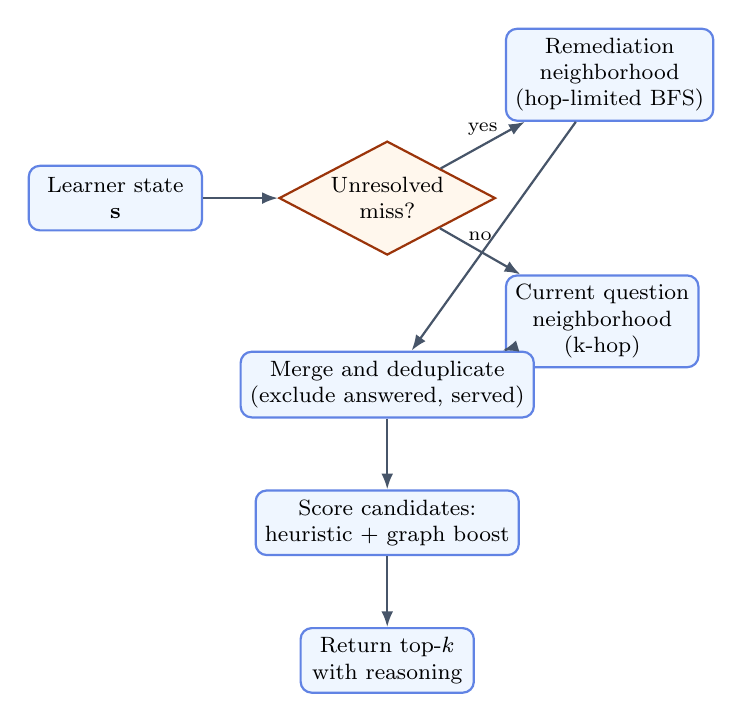
\begin{tikzpicture}[node distance=0.9cm and 0.95cm]
  \node[flow] (s) {Learner state\\$\mathbf{s}$};
  \node[decision, right=of s] (miss) {Unresolved\\miss?};
  
  \node[flow, above right=0.6cm and 0.8cm of miss] (remed) {Remediation\\neighborhood\\(hop-limited BFS)};
  \node[flow, below right=0.6cm and 0.8cm of miss] (current) {Current question\\neighborhood\\(k-hop)};
  
  \node[flow, below=1.2cm of miss] (candidate) {Merge and deduplicate\\(exclude answered, served)};
  \node[flow, below=of candidate] (score) {Score candidates:\\heuristic + graph boost};
  \node[flow, below=of score] (output) {Return top-$k$\\with reasoning};

  \draw[line] (s) -- (miss);
  \draw[line] (miss) -- node[above, font=\scriptsize]{yes} (remed);
  \draw[line] (miss) -- node[above, font=\scriptsize]{no} (current);
  \draw[line] (remed) -- (candidate);
  \draw[line] (current) -- (candidate);
  \draw[line] (candidate) -- (score);
  \draw[line] (score) -- (output);
\end{tikzpicture}
\caption{Adaptive recommendation pipeline decision logic.}
\end{figure}

\subsubsection{Remediation Neighborhood}
When a student answers a question incorrectly (unresolved miss), the engine defines a remediation neighborhood:

\begin{equation}
N_{\text{remed}}(q, h) = \{q' \in V : d_G(q, q') \leq h, \text{ not answered }, \text{ difficulty}(q') < \text{difficulty}(q)\}
\end{equation}

where $d_G(q, q')$ is the graph distance (hops), and $h$ (typically 2--3) is the maximum hop limit. This ensures:
\begin{itemize}
\item Questions are related to the originally missed question (nearby in graph).
\item But easier (to build confidence before retry).
\item And haven't been answered before.
\end{itemize}

\subsubsection{Current Question Neighborhood}
In standard (non-remediation) adaptive flow:

\begin{equation}
N_{\text{current}}(q, k) = \{q' \in V : d_G(q, q') \leq k, \text{ not answered }, \text{ not served }\}
\end{equation}

Typical $k = 2$ (2-hop neighbors).

\subsection{Candidate Scoring Function}

After assembling the candidate pool $C$, the engine scores each candidate $q' \in C$:

\begin{equation}
\text{score}(q') = w_h \cdot h(q') + w_g \cdot g(q')
\end{equation}

where:

\begin{itemize}
\item $h(q')$ is a \textbf{heuristic score} combining:
   \begin{enumerate}
   \item Distance to target difficulty: $d_{\text{diff}} = |\text{difficulty}(q') - \text{difficulty}_{\text{target}}|$
   \item Distance to target ELO: $d_{\text{elo}} = |\text{ELO}(q') - \text{ELO}_{\text{target}}|$
   \item Weak-topic bonus: if $q'$ is in a weak topic, add bonus $\beta_{\text{weak}}$.
   \item Type diversity: if $q'$ type differs from the current question, add bonus $\beta_{\text{type}}$.
   \end{enumerate}
   
   Typically:
   \begin{equation}
   h(q') = 1.0 - \frac{w_1 \cdot d_{\text{diff}} + w_2 \cdot d_{\text{elo}}}{C_{\text{norm}}} + \beta_{\text{weak}} \cdot \mathbb{1}[q' \in \text{weak\_topics}] + \beta_{\text{type}} \cdot \mathbb{1}[\text{type}(q') \neq \text{type}(q)]
   \end{equation}

\item $g(q')$ is a \textbf{graph boost} rewarding structural properties:
   \begin{equation}
   g(q') = \gamma_1 \cdot \rho_{\text{in}}(q') + \gamma_2 \cdot \rho_{\text{out}}(q') + \gamma_3 \cdot c(q')
   \end{equation}
   
   where:
   \begin{itemize}
   \item $\rho_{\text{in}}(q')$ = normalized in-degree (how many questions lead to $q'$).
   \item $\rho_{\text{out}}(q')$ = normalized out-degree (how many questions $q'$ leads to).
   \item $c(q')$ = normalized centrality measure (e.g., betweenness centrality).
   \end{itemize}
   
   Nodes with high centrality are pedagogically important \"hub\" questions, reflecting well-established learning pathways.
\end{itemize}

Weights $w_h$, $w_g$, and coefficients are tuned empirically via A/B testing or offline replay.

\subsection{Output and Explainability}

The engine returns the top-$k$ (typically $k=1$) candidate with:

\begin{itemize}
\item Question ID and full metadata (text, options, marks, expected difficulty).
\item Natural-language explanation: e.g., "Continuing on Linear Algebra---the next question is harder to strengthen your eigenvalue skills."
\item Graph metadata: hop distance, centrality signal, neighborhood type (remediation vs. standard).
\item Target ELO and expected difficulty for transparency.
\end{itemize}

\section{Remediation and Retry Engine}

When a student submits an incorrect answer, the system marks the question as an unresolved miss. The remediation engine manages the recovery process:

\subsection{Remediation Workflow}

\begin{equation}
\boxed{\begin{array}{l}
(1) \quad \text{Flag question as unresolved miss} \\
(2) \quad \text{Serve remediation neighbors (easier, related)} \\
(3) \quad \text{Track accuracy and step count within remediation sequence} \\
(4) \quad \text{After } N_{\text{remed}} \text{ successful steps or accuracy} \geq A_{\text{remed}}: \text{ unlock retry of original} \\
(5) \quad \text{If retry is correct: clear miss, mark as resolved} \\
(6) \quad \text{If retry is incorrect: re-queue for remediation}
\end{array}}
\end{equation}

\subsection{Remediation Exit Criteria}

Remediation concludes when:

\begin{equation}
\text{steps\_taken} \geq N_{\text{remed}} \quad \land \quad \text{remediation\_accuracy} \geq A_{\text{remed}}
\end{equation}

Typical values: $N_{\text{remed}} = 3$ remediation steps, $A_{\text{remed}} = 0.75$ (75\% accuracy).

If these criteria are not met within a session, the miss carries forward; the retry is queued for the next session.

\section{Practice Review and Rapid-Guess Detection Engine}

\subsection{Motivation: Quality of Evidence}
Not all correct answers represent equal mastery. A student might answer a complex multi-step problem correctly but in 10 seconds---suspicious and likely guessing. The rapid-guess detection engine in \tech{src/lib/practiceReview.ts} flags such scenarios.

\subsection{Threshold Computation}
For each question, the engine estimates a base minimum solve time:

\begin{equation}
t_{\text{min}}(q) = \alpha_0 + \alpha_1 \cdot \text{stem\_length}(q) + \alpha_2 \cdot \text{options\_length}(q) + \alpha_3 \cdot \text{complexity\_index}(q)
\end{equation}

where complexity index is higher for questions labeled as multi-step or requiring computation.

Typical coefficient values (empirically tuned):
\begin{itemize}
\item $\alpha_0 = 10$ seconds (baseline reading time).
\item $\alpha_1 = 0.02$ seconds per character in stem.
\item $\alpha_2 = 0.01$ seconds per character in option set.
\item $\alpha_3 = 30$ seconds for high-complexity questions.
\end{itemize}

\subsection{Penalty Application}

If $t_{\text{spent}}(q) < t_{\text{min}}(q)$:

\begin{equation}
\text{ELO\_penalty} = (1 - \frac{t_{\text{spent}}}{t_{\text{min}}}) \cdot 20 \text{ points}
\end{equation}

\begin{equation}
\text{ELO\_gain}(q) = \max(0, \text{standard\_gain} - \text{ELO\_penalty})
\end{equation}

The student still receives marks, but their ELO gain is reduced, preventing rapid guessing from inflating proficiency ratings.

\section{Coach Engine}

\subsection{Purpose and Scope}
The coach provides personalized study recommendations, learning plans, and guidance to students. Rather than being a chatbot, it focuses on structured, actionable coaching:

\begin{itemize}
\item Identifies weak and strong subject areas.
\item Recommends topic prioritization and revision strategies.
\item Generates same-day, 3-day, and 7-day study plans.
\item Provides mock preparation strategies and effort allocation advice.
\item Responds to student questions with carefully crafted rule-based recommendations.
\end{itemize}

\subsection{Rule-Based Implementation Architecture}

The coach is built on a pure rule-based heuristic engine with no external dependencies. All coaching logic is hand-crafted and parameterized based on empirical observations from GATE DA preparation patterns.

\textbf{Key Properties}:
\begin{enumerate}
\item \textbf{Fast Execution}: Response generation completes in milliseconds, ensuring responsive user experience.

\item \textbf{Deterministic and Explainable}: Every recommendation follows transparent, understandable rules that can be audited and explained to students.

\item \textbf{No External Dependencies}: The coach operates offline and does not require API calls, network connectivity, or external services.

\item \textbf{Custom Tuning}: Parameters are adjusted based on observed student behavior patterns within the platform.
\end{enumerate}

\subsection{Coach Input State}

The coach receives:

\begin{equation}
\mathbf{c} = (\text{ELO}, \text{tier}, \text{overall\_acc}, \text{weak\_subjects}, \text{strong\_subjects}, \text{streak}, \text{recent\_tests}, \text{focus\_area})
\end{equation}

where:
\begin{itemize}
\item $\text{ELO} \in [0, 3000]$: Current proficiency.
\item $\text{tier}$: Categorical proficiency level (Bronze, Silver, Gold, Platinum).
\item $\text{overall\_acc} \in [0, 1]$: Fraction of all questions answered correctly.
\item $\text{weak\_subjects}$: Set of subjects with accuracy $< \tau_{\text{weak}}$.
\item $\text{strong\_subjects}$: Set of subjects with accuracy $\geq \tau_{\text{strong}}$.
\item $\text{streak}$: Current correct-answer streak length.
\item $\text{recent\_tests}$: List of recent test results (score, accuracy, time).
\item $\text{focus\_area}$: Student-specified topic of interest or concern.
\end{itemize}

\subsection{Deterministic Coach Logic}

The fallback coach implements heuristic rules:

\subsubsection{Daily Study Suggestion}
\begin{equation}
\text{suggestion} = \begin{cases}
\text{``Focus on } w_1 \text{ today---you have } (100 - \text{acc}_{w_1})\% \text{ room for improvement.''} & \text{if weak\_subjects not empty} \\
\text{``Great momentum! Tackle harder problems in } s_1 \text{ today.''} & \text{if streak} > 5 \\
\text{``Review fundamentals in } w_1 \text{ to build confidence.''} & \text{otherwise}
\end{cases}
\end{equation}

\subsubsection{7-Day Study Plan}
The coach allocates effort across weak, strong, and new topics:

\begin{equation}
\boxed{\begin{array}{l}
\text{Day 1-2}: \text{Weak topic 1} \quad (40\% \text{ effort}) \\
\text{Day 3-4}: \text{Weak topic 2} \quad (30\% \text{ effort}) \\
\text{Day 5-6}: \text{Strong topic (mock)} \quad (20\% \text{ effort}) \\
\text{Day 7}: \text{Revision or new topic} \quad (10\% \text{ effort})
\end{array}}
\end{equation}

Effort allocation is parameterized by tier and recent performance.

\subsection{Coach Reasoning Logic}

The rule-based engine employs a multi-step pipeline to generate recommendations:

\subsubsection{Step 1: Student Profile Analysis}
The system analyzes the student input state to compute:
\begin{itemize}
\item Proficiency level based on current ELO (low: <1800, medium: 1800-2200, high: >2200).
\item Performance stability (comparing recent vs. historical accuracy).
\item Effort allocation efficiency (questions per topic studied).
\item Motivation signal (streak length and session frequency).
\end{itemize}

\subsubsection{Step 2: Weakness Severity Ranking}
Weak subjects are ranked by severity:
\begin{equation}
\text{severity}(s) = (1 - \text{accuracy}(s)) \times \text{weight}(s)
\end{equation}
where weight reflects importance in GATE DA (e.g., probability gets higher weight than niche topics).

\subsubsection{Step 3: Personalized Recommendations}
Based on the student profile, the coach selects from a curated set of advice templates:
\begin{itemize}
\item If ELO $< 1800$ and accuracy $< 50\%$: Focus on fundamentals and concept clarity.
\item If ELO $\in [1800, 2200]$ and improving: Maintain momentum by tackling harder questions.
\item If ELO $> 2200$ and accuracy $> 75\%$: Shift focus to speed optimization and mock practice.
\item If declining trend detected: Recommend topic-specific review and reduced difficulty.
\end{itemize}

\subsubsection{Step 4: Study Plan Generation}
The 7-day plan is constructed by:
\begin{itemize}
\item Day 1-2: Highest-severity weak topic (primary focus).
\item Day 3: Second-highest-severity weak topic and foundational concepts.
\item Day 4-5: Integrated practice covering multiple topics.
\item Day 6: Mock test or full-paper attempt to assess integrated readiness.
\item Day 7: Targeted revision of mistakes from the mock test.
\end{itemize}

Each day's plan includes specific exercise counts, difficulty targets, and expected study duration.

\section{Teacher Analytics and Intervention Intelligence} \label{sec:teacher-analytics}

\subsection{Teacher Workspace Aggregation}

The teacher workspace hook (in \tech{hooks/useTeacherWorkspace.ts}) aggregates classroom data:

\begin{enumerate}
\item Fetch all teaching credentials for the logged-in teacher.
\item Query all courses created by the teacher.
\item For each course, fetch enrollments, assignments, and submissions.
\item Execute a joined query over \tech{public} and \tech{teacher} schemas to retrieve student profiles, progress, test history, and activity events for enrolled learners.
\end{enumerate}

This creates a unified view of classroom state available to the teacher dashboard.

\subsection{Teacher Summary Computations}

\subsubsection{Student Summaries}

For each enrolled student, compute:

\begin{table}[H]
\centering
\small
\begin{tabular}{>{\raggedright\arraybackslash}p{0.3\columnwidth} >{\raggedright\arraybackslash}p{0.65\columnwidth}}
\toprule
\textbf{Metric} & \textbf{Definition} \\
\midrule
Overall Accuracy & $\text{acc} = \frac{\text{\# correct answers}}{\text{\# total answered}}$ \\
ELO & Current rating from \tech{profiles} \\
Weak Topics (top 3) & Subjects with accuracy $< 0.6$, sorted by severity \\
Assignment Completion & Fraction of assigned questions submitted \\
Risk Level & Composite score (see Section \ref{sec:risk-scoring}) \\
Recent Activity & Last action timestamp (question answered, test completed, etc.) \\
Performance Trend & 7-day accuracy comparison \\
\bottomrule
\end{tabular}
\caption{Student summary metrics computed for teacher viewing.}
\end{table}

\subsubsection{Course Summaries}

For each course, compute:

\begin{itemize}
\item Enrollment count: number of enrolled students.
\item Average accuracy: mean of all student accuracies.
\item Completion rate: fraction of assigned questions completed.
\item Weak topics (class-wide): frequency of below-threshold accuracy by subject.
\item At-risk student count: students with risk level $> T_{\text{risk}}$ (typically 0.7).
\item Top performers: students with accuracy $> T_{\text{top}}$ (typically 0.8).
\end{itemize}

\subsection{Risk Scoring} \label{sec:risk-scoring}

Risk distills learner challenges into a single actionable score. The composite risk score is:

\begin{equation}
\text{Risk}(s) = w_1 \cdot r_{\text{acc}}(s) + w_2 \cdot r_{\text{comp}}(s) + w_3 \cdot r_{\text{elo}}(s)
\end{equation}

where:

\begin{itemize}
\item $r_{\text{acc}}(s) = 1 - \text{accuracy}(s)$: Accuracy-based risk (lower accuracy = higher risk).
\item $r_{\text{comp}}(s) = 1 - \text{completion\_rate}(s)$: Completion-based risk (not engaging enough).
\item $r_{\text{elo}}(s) = \begin{cases} 1 & \text{if } \text{ELO}(s) < 1800 \\ 0 & \text{otherwise} \end{cases}$: ELO readiness (students under threshold need support).
\end{itemize}

Typical weights: $w_1 = 0.5$, $w_2 = 0.3$, $w_3 = 0.2$ (accuracy is the primary risk signal).

Students with $\text{Risk} \geq 0.7$ appear in the teacher's intervention queue.

\subsection{Intervention Recommendations}

For each at-risk student, the teacher analytics module recommends actions:

\begin{enumerate}
\item \textbf{Identify the top weak topic} with lowest accuracy.
\item \textbf{Suggest a targeted assignment}: author and publish an exercise within that weak topic.
\item \textbf{Check remediation progress}: query \tech{answered\_questions} to see if the student is successfully remediating past misses.
\item \textbf{Schedule a follow-up}: recommend a check-in date based on the assignment deadline.
\end{enumerate}

Example recommendation output:

\begin{verbatim}
Recommendation: Priya needs help with Probability & Statistics.
- Current accuracy: 45%
- Recent miss: Q2834 (binomial distribution)
- Suggested action: Publish a 5-question probability assignment
- Follow-up: Check progress in 2 days
\end{verbatim}

\section{GATE Score Prediction Engine} \label{sec:score-prediction}

\subsection{Vision and Purpose}

The GATE score prediction module \tech{src/components/GateScorePrediction.tsx} addresses a critical learner need: estimating likely final GATE scores based on current preparation progress. This enables students to:

\begin{itemize}
\item Set realistic targets (e.g., target 85+ percentile rank).
\item Allocate remaining study time effectively.
\item Identify whether their preparation pace is sufficient.
\item Build confidence through informed end-state projections.
\end{itemize}

\subsection{Unlock Criteria}

The score predictor is deliberately kept exclusive to avoid premature or unreliable predictions. It unlocks only when:

\begin{equation}
\text{Predictor UNLOCKED} \iff \begin{cases}
\text{ELO} \geq 2500 \quad \text{AND} \\
\text{full\_mock\_completion} \geq 0.70 \quad \text{AND} \\
\text{topic\_wise\_completion} \geq 0.70 \quad \text{AND} \\
\text{adaptive\_completion} \geq 0.70
\end{cases}
\end{equation}

This ensures the model operates on substantial evidence:
\begin{itemize}
\item ELO 2500+ indicates solid proficiency.
\item 70\% completion across all three learning modes ensures broad coverage and engagement depth.
\end{itemize}

\subsection{Core Formula: Predicted Score Basis}

Once unlocked, the predictor generates a \textbf{score basis}---a normalized composite score from four key dimensions:

\begin{equation}
\text{ScoreBasis} = w_1 \cdot \text{Acc}_{\text{norm}} + w_2 \cdot \text{ELO}_{\text{norm}} + w_3 \cdot \text{Cons}_{\text{norm}} + w_4 \cdot \text{Impr}_{\text{norm}}
\end{equation}

where the weights are: $w_1 = 0.40$, $w_2 = 0.30$, $w_3 = 0.20$, $w_4 = 0.10$.

Below, we explain each component in detail.

\subsubsection{Component 1: Overall Accuracy ($\text{Acc}$)}

\textbf{Conceptual Definition}:
\begin{equation}
\text{Accuracy} = \frac{\text{\# questions answered correctly}}{\text{\# total questions answered}}
\end{equation}

\textbf{Variable Definitions}:
\begin{itemize}
\item $C$: Count of correct answers (from \tech{answered\_questions} where \tech{is\_correct}=true).
\item $T$: Total questions answered.
\item $\text{Accuracy}_{raw} = \frac{C}{T}$.
\end{itemize}

\textbf{Normalization}:
\begin{equation}
\text{Acc}_{\text{norm}} = \min\left(1.0, \frac{\text{Accuracy}_{raw} - 0.5}{0.35}\right)
\end{equation}

This maps raw accuracy to $[0, 1]$:
\begin{itemize}
\item Accuracy $\leq 50\%$ (struggling) $\to$ normalized score $\leq 0$.
\item Accuracy $= 85\%$ (strong) $\to$ normalized score $\approx 1.0$.
\item Accuracy $> 85\%$ $\to$ capped at 1.0.
\end{itemize}

The lower bound (50\%) reflects that random guessing on MCQC with 4 options yields ~25\% accuracy; 50\% is a meaningful threshold above guessing.

\subsubsection{Component 2: ELO Rating ($\text{ELO}_{\text{norm}}$)}

\textbf{Conceptual Definition}:
The ELO rating (from \tech{profiles}) reflects learner proficiency through wins and losses relative to question difficulty. Higher ELO = stronger learner.

\textbf{Variable Definitions}:
\begin{itemize}
\item $\text{ELO}_{current}$: Current ELO from user profile (range: 0—3000).
\item $\text{ELO}_{baseline} = 1600$: Starting ELO.
\item $\text{ELO}_{max} = 2800$: Typical maximum reached by very strong learners.
\end{itemize}

\textbf{Normalization}:
\begin{equation}
\text{ELO}_{\text{norm}} = \frac{\text{ELO}_{current} - \text{ELO}_{baseline}}{\text{ELO}_{max} - \text{ELO}_{baseline}} = \frac{\text{ELO}_{current} - 1600}{1200}
\end{equation}

This maps:
\begin{itemize}
\item ELO = 1600 (baseline) $\to$ 0.0.
\item ELO = 2400 (strong) $\to$ 0.667.
\item ELO = 2800 (very strong) $\to$ 1.0.
\end{itemize}

\subsubsection{Component 3: Subject Consistency ($\text{Cons}_{\text{norm}}$)}

\textbf{Conceptual Definition}:
A learner with wildly varying subject accuracies (e.g., 90\% in one subject, 40\% in another) is less prepared than one with balanced proficiency. Consistency measures how evenly performance is distributed across subjects.

\textbf{Variable Definitions}:
\begin{itemize}
\item $S = \{s_1, s_2, \ldots, s_n\}$: Set of subjects (e.g., Linear Algebra, DBMS, Probability, ML, AI).
\item $\text{acc}_i = $ accuracy in subject $s_i$ (from \tech{user\_progress}).
\item $\bar{\text{acc}} = \frac{1}{n} \sum_{i=1}^{n} \text{acc}_i$: Mean accuracy across subjects.
\end{itemize}

\textbf{Consistency Metric (Inverse Coefficient of Variation)}:
\begin{equation}
\text{Consistency}_{raw} = 1 - \frac{\sigma(\text{acc}_1, \ldots, \text{acc}_n)}{\bar{\text{acc}} + \epsilon}
\end{equation}

where $\sigma$ is standard deviation and $\epsilon$ is a small value (e.g., 0.01) to avoid division by zero.

Intuitively:
\begin{itemize}
\item If all subjects have accuracy 75\%: $\sigma = 0 \Rightarrow$ Consistency = 1.0 (perfect).
\item If accuracies are [90\%, 40\%, 70\%, 65\%, 60\%], $\sigma$ is large $\Rightarrow$ Consistency is lower.
\end{itemize}

\textbf{Normalization}:
\begin{equation}
\text{Cons}_{\text{norm}} = \max(0, \text{Consistency}_{raw})
\end{equation}

Bounded to $[0, 1]$.

\textbf{Interpretation}:
A student with 80\% overall accuracy will score higher if that 80\% is evenly distributed (75\%, 85\%, 78\%, 82\%) vs. skewed (95\%, 45\%, 80\%, 85\%). The former shows better mastery of breadth; the latter shows gaps that may cause score loss in the actual exam.

\subsubsection{Component 4: Improvement Factor ($\text{Impr}_{\text{norm}}$)}

\textbf{Conceptual Definition}:
Students showing upward performance trends (improving over time) are likely to maintain or extend that improvement. The improvement factor rewards recent accelerating progress.

\textbf{Variable Definitions}:
\begin{itemize}
\item $T_{\text{recent}} \in (0, T_{\text{all}}]$: Recent time window (e.g., last 14 days).
\item $\text{acc}_{\text{recent}}$: Accuracy in recent window.
\item $\text{acc}_{\text{prior}}$: Accuracy in all prior data.
\item $\Delta \text{acc} = \text{acc}_{\text{recent}} - \text{acc}_{\text{prior}}$: Improvement magnitude.
\end{itemize}

\textbf{Improvement Metric}:
\begin{equation}
\text{Improvement}_{raw} = \begin{cases}
\min(0.15, \Delta \text{acc}) & \text{if } \Delta \text{acc} > 0 \quad \text{(improving)} \\
\max(-0.15, \Delta \text{acc}) & \text{if } \Delta \text{acc} \leq 0 \quad \text{(declining)}
\end{cases}
\end{equation}

This captures improvements/declines up to ±15 percentage points.

\textbf{Normalization}:
\begin{equation}
\text{Impr}_{\text{norm}} = \frac{\text{Improvement}_{raw} + 0.15}{0.30}
\end{equation}

Maps to $[0, 1]$:
\begin{itemize}
\item $\Delta \text{acc} = -15\%$ (declining) $\to$ 0.0.
\item $\Delta \text{acc} = 0\%$ (stable) $\to$ 0.5.
\item $\Delta \text{acc} = +15\%$ (improving) $\to$ 1.0.
\end{itemize}

\textbf{Interpretation}:
A student improving by 5 percentage points recently is rewarded; one declining is penalized. This captures momentum.

\subsection{Score Band Generation from Basis}

Once $\text{ScoreBasis} \in [0, 1]$ is computed, the predictor generates GATE score estimates. The GATE DA exam scoring is typically:

\begin{itemize}
\item Total marks: 100 (occasionally 85 or 90 depending on exam).
\item Question distribution: usually 55 MCQ (1 mark each) + 10 NAT (numerical) questions (various marks).
\end{itemize}

For simplicity, assume 100-mark scale.

\subsubsection{Expected Score}
\begin{equation}
\text{Expected\_Score} = 40 + 50 \cdot \text{ScoreBasis}
\end{equation}

This maps ScoreBasis to an expected GATE score:
\begin{itemize}
\item ScoreBasis = 0.0 (barely qualifying) $\to$ Expected = 40.
\item ScoreBasis = 0.5 (moderate) $\to$ Expected = 65.
\item ScoreBasis = 1.0 (excellent) $\to$ Expected = 90.
\end{itemize}

\subsubsection{Minimum and Maximum Score Bands}

To provide a confidence range, the model estimates bounds:

\begin{equation}
\text{Minimum\_Score} = \text{Expected\_Score} - 10 \cdot (1 - \text{ScoreBasis})
\end{equation}

\begin{equation}
\text{Maximum\_Score} = \text{Expected\_Score} + 10 \cdot \text{ScoreBasis}
\end{equation}

Intuitively:
\begin{itemize}
\item High ScoreBasis (near 1.0) $\to$ tight band (high confidence).
\item Low ScoreBasis (near 0.0) $\to$ wider band (more uncertainty).
\end{itemize}

Example:
\begin{itemize}
\item ScoreBasis = 0.8 $\Rightarrow$ Expected = 80, Min = 72, Max = 88.
\item ScoreBasis = 0.4 $\Rightarrow$ Expected = 60, Min = 46, Max = 64.
\end{itemize}

\subsubsection{Confidence Score}

Confidence reflects certainty in the prediction:

\begin{equation}
\text{Confidence} = 0.5 + 0.4 \cdot \text{ScoreBasis} + 0.1 \cdot \text{Completion\_Rate}
\end{equation}

where Completion\_Rate is the fraction of all GATE DA questions answered (0 to 1).

This maps to:
\begin{itemize}
\item Strong basis + high completion $\to$ Confidence near 1.0 (very confident).
\item Weak basis + low completion $\to$ Confidence near 0.5 (moderate confidence).
\end{itemize}

\subsubsection{Recommendation Text}

The predictor generates contextual guidance:

\begin{equation}
\text{RecommendationText} = \begin{cases}
\text{``Excellent! With your current preparation, expect GATE score 80--90.} \\ 
\text{Focus on maintaining consistency across all topics.''} & \text{if } \text{Expected} \geq 75 \\
\\
\text{``Good progress. Expected score 60--70. Strengthen weak topics:} \\
\text{[weak subjects list]. Increase mock attempt frequency.''} & \text{if } 60 \leq \text{Expected} < 75 \\
\\
\text{``Your preparation is on track for 40--60. Accelerate study} \\
\text{intensity, especially in: [weak subjects]. Try 1 mock/week.''} & \text{if } \text{Expected} < 60
\end{cases}
\end{equation}

\subsection{Worked Example}

Assume a student with:
\begin{itemize}
\item Accuracy: 78\%.
\item ELO: 2350.
\item Subject accuracies: [85\%, 72\%, 70\%, 75\%, 80\%] (standard deviation: 6\%).
\item Mean: 76.4\%.
\item Consistency: $1.0 - \frac{0.06}{0.764 + 0.01} \approx 0.922$.
\item Recent accuracy (last 14 days): 82\%; all prior: 75\%; $\Delta \text{acc} = 7\%$.
\end{itemize}

\textbf{Normalization:}
\begin{itemize}
\item $\text{Acc}_{\text{norm}} = \min(1.0, \frac{0.78 - 0.5}{0.35}) = \frac{0.28}{0.35} \approx 0.80$.
\item $\text{ELO}_{\text{norm}} = \frac{2350 - 1600}{1200} \approx 0.625$.
\item $\text{Cons}_{\text{norm}} = 0.922 \approx 0.92$.
\item $\text{Impr}_{\text{norm}} = \frac{0.07 + 0.15}{0.30} \approx 0.73$.
\end{itemize}

\textbf{Score Basis:}
\begin{equation}
\text{ScoreBasis} = 0.40 \cdot 0.80 + 0.30 \cdot 0.625 + 0.20 \cdot 0.92 + 0.10 \cdot 0.73
\end{equation}
\begin{equation}
= 0.32 + 0.1875 + 0.184 + 0.073 = 0.7645
\end{equation}

\textbf{Score Predictions:}
\begin{itemize}
\item Expected: $40 + 50 \cdot 0.7645 = 40 + 38.225 = 78.2 \approx 78$.
\item Minimum: $78 - 10 \cdot (1 - 0.7645) = 78 - 2.355 = 75.6 \approx 76$.
\item Maximum: $78 + 10 \cdot 0.7645 = 78 + 7.645 = 85.6 \approx 86$.
\item Confidence: $0.5 + 0.4 \cdot 0.7645 + 0.1 \cdot 0.70 \approx 0.5 + 0.306 + 0.07 = 0.876$ (high confidence).
\end{itemize}

\textbf{Recommendation:}
"Good progress. Expected GATE score: 76--86 (best estimate: 78). Consistency is strong across topics. Recent acceleration (+7\%) is encouraging---maintain this pace by continuing daily practice on weak areas."

\section{Deployment and Network Configuration}

\subsection{Supabase Configuration and Setup}

The \project{} platform relies on Supabase as its backend infrastructure. The configuration is managed through environment variables defined in the \tech{.env} file:

\begin{table}[H]
\centering
\small
\begin{tabular}{>{\raggedright\arraybackslash}p{0.35\columnwidth} >{\raggedright\arraybackslash}p{0.6\columnwidth}}
\toprule
\textbf{Environment Variable} & \textbf{Purpose} \\
\midrule
VITE\_STUDENT\_SUPABASE\_PROJECT\_ID & Project identifier for student-facing services \\
VITE\_STUDENT\_SUPABASE\_URL & REST API endpoint for student data access \\
VITE\_STUDENT\_SUPABASE\_PUBLISHABLE\_KEY & Public API key for unauthenticated operations \\
VITE\_TEACHER\_SUPABASE\_PROJECT\_ID & Project identifier for teacher-facing services \\
VITE\_TEACHER\_SUPABASE\_URL & REST API endpoint for teacher/classroom data \\
VITE\_TEACHER\_SUPABASE\_PUBLISHABLE\_KEY & Public API key for teacher operations \\
VITE\_TEACHER\_SUPABASE\_SCHEMA & Database schema targeting (default: public) \\
\bottomrule
\end{tabular}
\caption{Environment variables for Supabase connectivity.}
\end{table}

\subsection{Network Connectivity Troubleshooting}

\subsubsection{Common Connection Issues}

The platform implements robust error handling for common network scenarios:

\begin{enumerate}
\item \textbf{Connection Reset Errors}: When Supabase server forcibly closes connections (error 10054 on Windows), typically due to:
   \begin{itemize}
   \item Network firewall or proxy blocking HTTPS traffic.
   \item Supabase service experiencing temporary outages.
   \item Invalid or expired project credentials.
   \item Regional connectivity issues (attempting to reach a geographically distant server).
   \end{itemize}

\item \textbf{Timeout Errors}: Requests exceed response time limits (default 10-15 seconds), indicating:
   \begin{itemize}
   \item Slow network connection or high latency.
   \item Supabase server overload or degradation.
   \item Large query result sets causing serialization delays.
   \end{itemize}

\item \textbf{Unauthorized (401) Errors}: API key is invalid or RLS policies deny access:
   \begin{itemize}
   \item Public key has insufficient permissions for queried tables.
   \item Row-Level Security (RLS) policies require JWT authentication.
   \item User session token has expired.
   \end{itemize}

\item \textbf{Not Found (404) Errors}: Queried table or endpoint does not exist:
   \begin{itemize}
   \item Supabase schema migration incomplete.
   \item Table name mismatch between code and database.
   \item API endpoint version mismatch.
   \end{itemize}
\end{enumerate}

\subsubsection{Diagnostic and Recovery Procedures}

The \tech{STUDENT\_PROGRESS\_TRACKER.ipynb} notebook includes a comprehensive diagnostic cell that:

\begin{enumerate}
\item Verifies environment variables are correctly loaded from \tech{.env}.
\item Tests connectivity with a simple query (limit=1) to detect basic connectivity issues.
\item Logs detailed request/response information for debugging.
\item Categorizes errors into actionable resolution steps.
\end{enumerate}

\textbf{Diagnostic Checklist}:

\begin{verbatim}
1. ✅ Environment Variables Loaded
   - Check VITE_STUDENT_SUPABASE_URL is not empty
   - Verify VITE_STUDENT_SUPABASE_PUBLISHABLE_KEY is valid (>20 chars)
   
2. 📡 Network Connectivity
   - Verify internet connection is active
   - Check firewall/proxy is not blocking *.supabase.co domains
   - Try alternate DNS (e.g., 8.8.8.8)
   
3. 🔑 Authentication
   - Confirm API key corresponds to correct Supabase project
   - Verify project URL matches: https://[PROJECT_ID].supabase.co
   - Check RLS policies allow public key access to tables
   
4. 📊 Database Readiness
   - Verify all required tables exist in database
   - Confirm schema migrations have completed
   - Test with curl/Postman before running Python notebook
\end{verbatim}

\subsubsection{Connection Resilience Strategy}

The fetch functions implement exponential backoff retry logic:

\begin{equation}
\text{wait\_time} = \text{base\_delay} \times (1 + \text{jitter})^{\text{attempt\_number}}
\end{equation}

where:
\begin{itemize}
\item $\text{base\_delay}$ = 1 second (initial retry delay).
\item $\text{jitter} \in [0, 1)$ = random jitter to avoid thundering herd.
\item $\text{attempt\_number} \in [0, 2]$ = retry count (3 total attempts).
\end{itemize}

Example progression:
\begin{itemize}
\item Attempt 1 fails: wait 1 second, retry.
\item Attempt 2 fails: wait 1-2 seconds, retry.
\item Attempt 3 fails: return empty dataset, fall back to mock data.
\end{itemize}

This ensures transient network hiccups don't cause immediate failures, while permanent outages are detected quickly.

\subsection{Data Persistence Fallback Strategy}

When Supabase connectivity is unavailable, the platform implements graceful degradation:

\begin{enumerate}
\item \textbf{Local State Preservation}: React Query caches are persisted to browser localStorage, enabling read-only access to recently-viewed data.

\item \textbf{Mock Data Mode}: A fallback dataset (in \tech{src/data/mockData.ts}) provides realistic question bank and student profile samples for development and demonstration.

\item \textbf{Offline Queuing}: User actions (answers submitted, tests completed) are queued in indexedDB. Once connectivity restores, changes are synced to Supabase with conflict resolution.

\item \textbf{User Notification}: Clear messaging informs the user of limited connectivity:
   \begin{verbatim}
   ⚠️ Working Offline
   Some features are limited. Changes will sync when connection restores.
   \end{verbatim}
\end{enumerate}

\subsection{Supabase Architecture Best Practices}

\subsubsection{Row-Level Security (RLS) Policies}

All public schema tables enforce RLS:

\begin{equation}
\boxed{\begin{array}{l}
\text{profiles: } \text{users can view/edit only their own profile} \\
\text{user\_progress: } \text{users can view/edit only their own progress records} \\
\text{answered\_questions: } \text{users can view/edit only their own answers} \\
\text{test\_history: } \text{users can view their own tests; teachers can view enrolled students'} \\
\text{teacher schema: } \text{teachers have full access to own courses/assignments; students have read-only on enrollments}
\end{array}}
\end{equation}

RLS policies are enforced at the database layer, ensuring even compromised API keys cannot access unauthorized data.

\subsubsection{Connection Pooling and Performance}

Supabase REST API includes connection pooling and caching:

\begin{itemize}
\item HTTP/2 multiplexing reduces overhead for concurrent requests.
\item Supabase edge functions support request batching to reduce round trips.
\item Query responses are cached by Supabase CDN when appropriate (e.g., question bank read-only data).
\end{itemize}

For high-frequency operations (e.g., rapid question serving during adaptive sessions), batch requests are used to reduce latency:

\begin{equation}
\text{Time per request} = \text{network\_latency} + \text{database\_query\_time}
\end{equation}

Batching amortizes network latency:

\begin{equation}
\text{Cost (N requests batched)} < N \times \text{Cost (N individual requests)}
\end{equation}

\section{Telemetry, Persistence, and Event-Driven Observability}

\subsection{State Persistence Strategy}

The platform persists learner state in two forms:

\subsubsection{Persistent State (Tables)}
\begin{itemize}
\item ELO, tier, and profile metadata in \tech{profiles}.
\item Subject accuracy and weak-topic tracking in \tech{user\_progress}.
\item Complete answer history in \tech{answered\_questions} (for replay and remediation).
\item Test summaries with optional \tech{review\_payload} in \tech{test\_history}.
\end{itemize}

This state is queried by the recommendation engines, analytics modules, and student dashboards.

\subsubsection{Event Stream (activity\_events table)}
In addition to state, every significant action is logged as an event:

\begin{table}[H]
\centering
\small
\begin{tabular}{>{\raggedright\arraybackslash}p{0.25\columnwidth} >{\raggedright\arraybackslash}p{0.7\columnwidth}}
\toprule
\textbf{Event Type} & \textbf{Metadata} \\
\midrule
\tech{user\_signed\_up} & user\_id, email, timestamp \\
\tech{user\_signed\_in} & user\_id, timestamp \\
\tech{question\_answered} & user\_id, question\_id, is\_correct, time\_spent \\
\tech{test\_started} & user\_id, test\_type, test\_name \\
\tech{test\_completed} & user\_id, test\_type, score, accuracy \\
\tech{graph\_path\_started} & user\_id, session\_id \\
\tech{graph\_path\_completed} & user\_id, session\_id, questions\_count, accuracy \\
\tech{course\_joined} & user\_id, course\_id \\
\tech{course\_left} & user\_id, course\_id \\
\tech{assignment\_published} & teacher\_id, course\_id, assignment\_id \\
\tech{submission\_received} & student\_id, assignment\_id, score \\
\bottomrule
\end{tabular}
\caption{Sample activity events and associated metadata.}
\end{table}

\subsection{Why This Design Matters}

The dual stream (state + events) is critical:

\begin{enumerate}
\item \textbf{Explainability}: Given a student's current ELO, the event stream enables reconstruction of how they arrived at that rating (what answers led to ELO changes).

\item \textbf{Observability}: Teachers and administrators can inspect recent activity, understand student engagement patterns, and identify behavioral anomalies.

\item \textbf{Research and Analytics}: The event stream enables longitudinal studies, cohort analysis, and identification of effective learning sequences.

\item \textbf{Audit Trail}: Every significant action is recorded, supporting academic integrity monitoring.

\item \textbf{Dashboard and History Views}: Students can replay past sessions using the \tech{review\_payload}, understanding which questions they missed and why.
\end{enumerate}

\section{History Review and Explainable Replaying}

A salient feature is the \textbf{review\_payload} field in \tech{test\_history}. When a test completes, the system optionally records:

\begin{itemize}
\item List of question IDs presented (in order).
\item For each question: submitted answer, correctness, time spent, any rapid-guess warning.
\item ELO change due to the question (if available).
\item Explanation metadata (graph information, remediation notes).
\end{itemize}

This enables a \textbf{replayable history view}:

\begin{enumerate}
\item Student selects a past test from history.
\item System reconstructs the session question-by-question.
\item For each question, the app displays: question text, student's answer, correct answer, explanation.
\item Rapid-guess warnings are highlighted: "This was answered in 5 seconds, but estimated minimum was 12 seconds. ELO boost was reduced."
\end{enumerate}

This transforms history from opaque score summaries into interactive learning artifacts.

\section{Research Assets and Analytical Notebooks}

The repository includes Python-based analysis tools:

\begin{itemize}
\item \tech{generate\_gate\_da\_question\_graph\_notebook.py}: Creates a Jupyter notebook analyzing the question recommendation graph (centrality, connectivity, degree distribution).

\item \tech{generate\_gate\_da\_student\_progress\_notebook.py}: Generates a notebook with student cohort analytics (ELO distribution, accuracy trends, subject performance heatmaps).

\item Teacher dashboard mockup generator: Creates sample visualizations showing class-wide metrics.
\end{itemize}

These notebooks use the same data model and provide exploratory analysis complementary to the live UI.

\section{Testing and Quality Assurance}

\subsection{Test Coverage for Adaptive Engine}

The adaptive engine is the highest-risk component, so it receives focused testing:

\begin{enumerate}
\item \textbf{Same-Topic Progression}: After answering a question correctly, the next recommendation should be in the same topic but harder (or similar difficulty).

\item \textbf{Cross-Topic Remediation}: After answering incorrectly, remediation recommendations should be easier and preferably in the same topic.

\item \textbf{Retry Logic}: After sufficient remediation with high accuracy, a retry of the missed question should be queued.

\item \textbf{Exclusion of Answered Questions}: Previously answered questions must never be served again in a session.

\item \textbf{ELO Bounds}: ELO changes must stay within expected ranges, and rapid-guess penalties must be correctly applied.
\end{enumerate}

Tests are written in Vitest with fixtures for sample graphs and learner states.

\subsection{Component Testing}

React components (especially recommendation displays and adaptive flows) are tested using Testing Library to ensure:

\begin{itemize}
\item Recommendations are rendered with rationale text.
\item Answer submission correctly updates state.
\item History replay correctly reconstructs past sessions.
\item Teacher dashboards correctly filter and display student data.
\end{itemize}

\subsection{E2E Testing}

Playwright tests cover end-to-end flows:

\begin{enumerate}
\item Student signup, login, and profile creation.
\item Joining a teacher course via code.
\item Attempting an adaptive session and verifying ELO updates.
\item Reviewing history and replaying answers.
\item Teacher viewing classroom dashboards and intervention recommendations.
\end{enumerate}

\section{Architectural Strengths}

\begin{enumerate}
\item \textbf{Clean Role Separation}: Student and teacher experiences are conceptually distinct, reflected in separate UI paths and data schemas.

\item \textbf{Explainable Recommendations}: Every recommendation includes reasoning (graph hop distance, difficulty target, weak-topic signal), supporting learner trust and educator understanding.

\item \textbf{Comprehensive Telemetry}: The \tech{activity\_events} stream enables observability into learner behavior, supporting debugging, analytics, and curiosity-driven research.

\item \textbf{Intelligent Rule-Based Coaching}: The coaching engine is built on carefully designed heuristics and domain knowledge, ensuring transparent, understandable, and reliable recommendations without external dependencies.

\item \textbf{Replayable History}: The \tech{review\_payload} upgrade converts static score records into interactive learning artifacts for deeper reflection.

\item \textbf{Remediation-Aware Sequencing}: The adaptive engine doesn't just select harder questions; it proactively identifies unresolved misses and queues targeted recovery sequences.

\item \textbf{Teacher-Centric Actional Insights}: Analytics output prioritizes actionable recommendations (suggest specific assignments, identify at-risk students) over passive reporting.

\item \textbf{Thoughtful Score Prediction}: The GATE score predictor balances mathematical rigor (detailed formula with four normalized components) with practical utility (confidence bands, recommendation text).

\item \textbf{Research Layer}: Python notebooks and analysis tooling complement the live UI, supporting exploratory analytics and academic inquiry.
\end{enumerate}

\section{Limitations and Future Enhancements}

\subsection{Current Limitations}

\begin{enumerate}
\item \textbf{Formal Experiment Tracking}: The platform lacks a first-class A/B testing framework. Recommendation policy changes are not yet systematically compared via randomized experiments.

\item \textbf{Longitudinal In-App Analytics}: While the \tech{activity\_events} stream is rich, fewer longitudinal visualizations are surfaced directly in the app. Most longitudinal analysis happens in notebooks.

\item \textbf{Score Prediction History}: Current predictions are point-in-time. Persisting historical predictions would enable trend analysis (``How did my predicted score change over the past month?'').

\item \textbf{Spaced Repetition}: The remediation engine is reactive (triggered after misses). A proactive spaced-repetition system would queue forgotten topics for revisiting.

\item \textbf{Prerequisite Graphs}: The current graph is similarity-based. An explicit prerequisite graph (e.g., Linear Algebra Fundamentals $\to$ Eigenvalues) would improve sequencing.

\item \textbf{Cross-Subject Integration}: While the graph includes subject-bridge edges, deeper integrative questions (combining multiple subjects) are underrepresented.
\end{enumerate}

\subsection{Recommended Enhancements}

\begin{enumerate}
\item \textbf{A/B Testing Framework}: Implement experiment tracking so that recommendation engine variants can be systematically compared on engagement, learning gain, and score prediction accuracy.

\item \textbf{Spaced Repetition Scheduler}: Integrate a Leitner-box style system for proactive weak-topic revisiting at optimal intervals.

\item \textbf{Prerequisite Awareness}: Explicitly model prerequisites and enforce sequencing (don't serve eigenvalue questions until linear-solve fundamentals are mastered).

\item \textbf{In-App Longitudinal Dashboards}: Display student ELO trends, weak-topic evolution, and predicted score trajectory directly in student and teacher dashboards.

\item \textbf{Adaptive Difficulty Calibration}: Use item-response theory (IRT) to calibrate question difficulties and adapt them based on population performance.

\item \textbf{Peer Benchmarking}: Compare student performance against class cohort (anonymous) to provide contextualized feedback.

\item \textbf{Intelligent Content Recommendation}: Beyond questions, recommend:
   \begin{itemize}
   \item Reading materials or videos for weak topics.
   \item Worked examples and step-by-step solutions.
   \item Similar previously-solved questions for reinforcement.
   \end{itemize}

\item \textbf{Real-Time Collaboration Features}: Enable peer study groups, shared notes, and instructor office hours within the platform.
\end{enumerate}

\section{Conclusion}

\project{} is a comprehensive, multi-dimensional educational intelligence platform that transcends simple mock-test portals. Its core value lies not in any single component, but in the seamless integration of:

\begin{itemize}
\item \textbf{Graph-based adaptive sequencing} that personalizes question difficulty and topic selection.
\item \textbf{Multiple specialized recommendation engines} addressing next-best questions, remediation, rapid-guess detection, and personalized coaching.
\item \textbf{Classroom orchestration tools} enabling teachers to author assignments, monitor progress, and receive intervention recommendations.
\item \textbf{Comprehensive telemetry} capturing both persistent state (ELO, scores) and event streams (actions, decisions) for deep observability.
\item \textbf{Predictive scoring} powered by a rigorous, four-component formula that estimates likely GATE scores with confidence bands.
\item \textbf{Rule-based coaching system} that delivers personalized study recommendations and guidance based on student performance analysis.
\item \textbf{Explainable, replayable history} enabling students to revisit and learn from past attempts.
\item \textbf{Research and analytics infrastructure} supporting longitudinal studies and exploratory insights.
\end{itemize}

This combination positions \project{} as a strong candidate for:

\begin{itemize}
\item \textbf{Advanced undergraduate or graduate project submissions}: Demonstrating systems integration, machine learning, and educational technology depth.
\item \textbf{Technical job portfolios}: Showcasing full-stack development, architectural thinking, and domain expertise.
\item \textbf{Academic research}: Publishing work on adaptive learning, recommendation systems, or educational analytics.
\item \textbf{StartUp/Product pitches}: Presenting a differentiated solution addressing real learner and educator needs.
\item \textbf{Viva and technical interviews}: Discussing complex systems, tradeoff decisions, and future research directions.
\end{itemize}

The platform demonstrates that educational software, when thoughtfully designed, can elevate not just test scores but learner autonomy, teacher effectiveness, and the quality of educational evidence.

\end{document}